\chapter{Theta Kernels, Fermion Determinants and Howe Duality}\label{ch:theta}\index{theta lift}\index{Howe duality}\index{fermion determinant}\index{colour flavour transformation}\index{matching polynomial}

\begin{quote}
\emph{A chain of theta lifts drives the argument for the Riemann hypothesis announced in November 2026, and our chapter on it in the Riemann volumes~\cite{PS26t} asks what part of the chain has a Thorin form. This chapter asks the same of Yang Mills. The answer is that the laws with real zeros of Chapter~\ref{ch:zeros} are products of fermion determinants, that their characters are theta lifts in the sense of Howe~\cite{Ho89}, and that decimation has an exact expansion over matchings.}
\end{quote}

\section{The question}

In \emph{Theta lifts and the Thorin programme} \cite{PS26t} we set the chain of theta lifts of the Alp\"oge and Claude proof, announced on 20 November 2026 with a Lean development \cite{Alp26}, beside the Thorin programme. Our reading of the argument rests on an unpublished account \cite{DLCL}, and we do not report any verdict on the proof. The archimedean half translates exactly: the statistic that the chain bounds is the cosine transform of the centre Thorin measure, its sharp constant is a Stieltjes transform, multiplicity is Thorin mass, the period term is $\log\Gamma$, and positivity of the Thorin measure at level $\alpha$ is the inequality $\operatorname{Re}\frac{\xi'}{\xi}(\alpha+is)\ge\frac{\xi'}{\xi}(\alpha)$. The arithmetic half, divisibility of theta values at finite places and the slope inequality that pays for it, has no counterpart there. Are theta lifts of use for the mass gap? Yang Mills has no finite places, so the arithmetic half has nothing to act on. The other half turns out to be already present in this book, under other names.

\section{Laws with real zeros are fermion determinants}\label{sec:t11det}

\begin{proposition}\label{prop:determinant}
For $U\in{}$SU(2) with eigenvalues $e^{\pm i\theta}$ and $0<\alpha\le1$,
\[
\det(1+\alpha U)=1+2\alpha\cos\theta+\alpha^2=2\alpha\,(\gamma+\cos\theta),\qquad\gamma=\frac{\alpha+\alpha^{-1}}2\ge1 .
\]
Hence the polynomials of the class $\mathcal L$ are exactly the functions $c\prod_{m=1}^d\det(1+\alpha_mU)$ with $0<\alpha_m\le1$: the zeros in $z=e^{i\theta}$ are $-\alpha_m^{\pm1}$, and the densities $f_j$ are $\det(1+U)^j$ normalised.
\end{proposition}

\begin{proof}
$(1+\alpha e^{i\theta})(1+\alpha e^{-i\theta})$.
\end{proof}

A determinant $\det(1+\alpha U)$ is the integral over one flavour of Grassmann variables in the fundamental representation, a heavy fermion of hopping parameter $\alpha$ running once round the plaquette. So a law with real zeros is the weight induced on a plaquette by $d$ fermion flavours with real hopping parameters, and the zeros of the law in $\cos\theta$ are the numbers $-\gamma_m$ fixed by the hopping parameters. Three things in the book read differently in this light.

\emph{The count is an occupation number.} $\det(1+\alpha U)=(1-\alpha)^2+\alpha\det(1+U)$, so each flavour is either inert or contributes a full factor $\det(1+U)$, and the latent count $M_0$ of Chapter~\ref{ch:counts} is the number of flavours of the second kind, a sum of independent Bernoulli variables as was found there.

\emph{The theta function is a free fermion.} By the proof of Theorem~\ref{thm:product} the theta function $\vartheta$ with $K_t=\frac12\partial_x\vartheta$ is $c\prod_{n\ge1}\det(1+q^{2n-1}U)$ with nome $q=e^{-t/4}$. This is the Jacobi triple product in its fermionic reading: a tower of flavours with hopping parameters $q,q^3,q^5,\dots$, the partition function of a free fermion on a circle twisted by $U$.

\emph{Bond moving is the multiplicity of the chain.} Raising a law to the power $k$ multiplies the number of flavours of each mass by $k$, and the Thorin measure of its reciprocal by $k$. That is the statement of \cite{PS26t} that multiplicity is Thorin mass, with bond moving playing the part of Stepanov's order of vanishing and of the length of the chain.

\section{Characters as a theta lift}\label{sec:t11howe}

Howe's duality \cite{Ho89} for the pair $(\mathrm{GL}_2,\mathrm{GL}_d)$ acting on the exterior algebra of $\mathbb C^2\otimes\mathbb C^d$ is the dual Cauchy identity $\prod_m\det(1+\alpha_mU)=\sum_\lambda s_\lambda(U)\,s_{\lambda'}(\alpha)$, the sum over partitions with at most two rows and at most $d$ columns. For SU(2) the Schur function $s_\lambda(U)$ with $\lambda=(\lambda_1,\lambda_2)$ is the character $\chi_n$ with $n=\lambda_1-\lambda_2+1$.

\begin{proposition}[characters from the flavour group]\label{prop:howe}
Let $f=\prod_{m=1}^d\det(1+\alpha_mU)=\sum_na_n\chi_n$. Then
\[
a_n=\sum_{j\ge0}s_{(2^j,1^{n-1})}(\alpha_1,\dots,\alpha_d)=\sum_{q\ge0}e_q(\alpha)\big(e_{q+n-1}(\alpha)-e_{q+n+1}(\alpha)\big),
\]
with $e_q$ the elementary symmetric functions. In particular every $a_n$ is a positive combination of characters of the flavour group evaluated at the hopping parameters.
\end{proposition}

\begin{proof}
The first form is the dual Cauchy identity, the conjugate of a partition with two rows being one with columns of length at most two. For the second, $f(z)=\prod_m(1+\alpha_mz)(1+\alpha_mz^{-1})=\sum_{p,q}e_pe_qz^{p-q}$, and $a_n$ is the coefficient of $z^n$ in $(z-z^{-1})f(z)$.
\end{proof}

So the Fourier transform on SU(2) that this book has used throughout, restricted to laws with real zeros, is a theta lift: it carries the diagonal element $\alpha$ of the flavour group to the sequence $(a_n)$ on the colour side, and the convolution theorem $a_nb_n/n$ is a statement about products of two such lifts divided by a dimension. With $d=3$ random hopping parameters the two sides of the proposition agree to all digits computed, $a=(8.189239,\ 8.007383,\ 3.302004,\ 0.520122)$.

\section{Decimation as a sum over matchings}\label{sec:t11match}

For unit quaternions $\det(V+\alpha U)=|V+\alpha U|^2$. Writing $v,u,e$ for the points of $S^3\subset\mathbb R^4$ that represent $V$, $U$ and the identity, with $u\cdot e=\cos\theta=x$, the convolution of two determinant laws is an integral over the sphere of a product of squared distances,
\[
(f*\psi)(x)=\int_{S^3}\prod_{m=1}^d\big|v+\alpha_mu\big|^2\prod_{k=1}^D\big|v+\kappa_ke\big|^2\,d\sigma(v).
\]
Two exact formulas follow.

\begin{lemma}[the ellipse]\label{lem:ellipse}
For class functions $f,\psi$ on SU(2) and $-1<x<1$, $(f*\psi)(x)$ is the average of $f(y_1)\,\psi(y_2)$ over the ellipse $y_1^2+y_2^2-2xy_1y_2\le1-x^2$ with respect to area.
\end{lemma}

\begin{proof}
$(f*\psi)(x)=E\,f(u\cdot v)\,\psi(e\cdot v)$ for $v$ uniform on $S^3$. The projection of the uniform law of $S^{n-1}$ on a plane has density proportional to $(1-|p|^2)^{(n-4)/2}$ on the disc, which is constant for $n=4$; the pair $(u\cdot v,e\cdot v)$ is a linear image of that projection, and the disc goes to the ellipse.
\end{proof}

\begin{theorem}[matching expansion]\label{thm:matching}
Let $f=\prod_{m=1}^d\det(1+\alpha_mU)$ and $\psi=\prod_{k=1}^D\det(1+\kappa_kU)$, and write $a_1,\dots,a_{d+D}$ for the hopping parameters of both. Then
\[
(f*\psi)(x)=\sum_{M}\frac{2^{|M|}}{(|M|+1)!}\ \prod_{i\notin M}\big(1+a_i^2\big)\prod_{\{i,j\}\in M}a_ia_j\ \ x^{c(M)},
\]
the sum over all matchings $M$ of the complete graph on the $d+D$ flavours, with $|M|$ the number of pairs and $c(M)$ the number of pairs that join a flavour of $f$ to a flavour of $\psi$.
\end{theorem}

\begin{proof}
Each factor is affine in $v$: $|v+\alpha u|^2=(1+\alpha^2)+2\alpha\,u\cdot v$. Expand the product, and use the moments of the uniform law on $S^{n-1}$,
\[
E\prod_{i=1}^{2k}(w_i\cdot v)=\frac{1}{n(n+2)\cdots(n+2k-2)}\sum_{\text{pairings}}\prod(w_i\cdot w_j),
\]
which for $n=4$ has the constant $1/\big(2^k(k+1)!\big)$. The inner products are $4a_ia_j$ for two flavours of the same law and $4a_ia_jx$ for flavours of different laws.
\end{proof}

For $d=D=1$ the theorem reads $(1+\alpha^2)(1+\kappa^2)+\alpha\kappa x$, which is the convolution computed from characters. For $d=3$ and $D=4$, a sum over the $232$ matchings of seven flavours, the two computations agree to six figures in every coefficient. The hypergeometric law of Theorem~\ref{thm:hypergeometric} is the case in which all hopping parameters are $1$.

The expansion puts the central conjecture of Chapter~\ref{ch:zeros} next to a classical theorem. Mark every pair by a variable $\tau$, so that $P(\tau,x)=\sum_M\tau^{|M|}x^{c(M)}w(M)$ with $w(M)$ the product of weights above. For fixed $x\ge0$ this is a matching polynomial of a graph with positive weights, and by the theorem of Heilmann and Lieb \cite{HL72} it has only real zeros in $\tau$; the factors $1/(|M|+1)!$ are a multiplier sequence of the first kind and keep them real. So in the variable that counts all pairs the reality of zeros is a theorem. Conjecture~\ref{conj:Lclosed} is the reality of zeros in the variable $x$ that counts only the pairs joining the two laws, with the pairs inside each law present and unmarked. If those inner pairs were absent, the two variables would coincide and the conjecture, as far as reality of zeros goes, would be the theorem of Heilmann and Lieb. They are present because SU(2) is a symplectic group: a flavour and its conjugate are equivalent, so two flavours of the same law can pair.

\paragraph{\normalfont\scshape The unitary group, and the colour flavour transformation.} For U(2) in place of SU(2) the inner pairs are absent, and Zirnbauer's colour flavour transformation \cite{Zi96}, which rests on Howe duality, turns the integral over the gauge group into an integral over a $d\times D$ complex matrix $Z$ of flavour variables. Carried out for our integrand it should give, if our recollection of \cite{Zi96} is right,
\[
\int_{\mathrm U(2)}\prod_m\det(1+\alpha_mUV^{-1})\prod_k\det(1+\kappa_kV)\,dV
=c\int\Phi_Z(U)\,\frac{dZ}{\det(1+ZZ^\dagger)^{d+D+2}},
\]
with $\Phi_Z(U)=\prod_i\det\big(1+\lambda_i(Z)\,U\big)$, where the $\lambda_i(Z)\ge0$ are the eigenvalues of $\alpha Z\kappa Z^\dagger$, with $\alpha$ and $\kappa$ the diagonal matrices of hopping parameters: the average over the unitary group of two determinant laws would be a positive mixture of determinant laws. We have checked this for one flavour each, where both sides are $1+\alpha\kappa x+\alpha^2\kappa^2$, and have not written out the general case; the transformation for SU(2) has further sectors, which are the inner pairs. Budczies and Zirnbauer \cite{BZ03} used the same duality to induce a lattice gauge theory from auxiliary bosons, whose plaquette weights are reciprocals of determinants, the Thorin side of the same class. A mixture of laws with real zeros need not have real zeros, so this does not prove the conjecture; it would say, for U(2), that decimation never leaves the convex hull of the class, and it names the mixing variable.

\section{The two programmes side by side}

\begin{center}
\small
\begin{tabular}{p{0.45\textwidth}p{0.47\textwidth}}
\toprule
theta chain and Thorin programme \cite{PS26t} & this book \\ \midrule
multiplicity is Thorin mass; $\varphi^m$ has $m$ times the Thorin measure of $\varphi$ & bond moving $\rho\mapsto\rho^k$ multiplies the flavours and the Thorin atoms by $k$ \\
a chain of positive kernels on a genus & the ladder, a chain of positive kernels on counts \\
Jacobi's theta function is a generalized gamma convolution \cite{BPY,Bo92} & the heat kernel is a product of fermion determinants; its reciprocal has Thorin atoms at the $\gamma_m$ \\
Thorin density at level $\alpha$: $\operatorname{Re}\frac{\xi'}{\xi}(\alpha+is)\ge\frac{\xi'}{\xi}(\alpha)$, open & Thorin density of the Hartman Watson law \cite{HW74}: $\operatorname{Re}\partial_\nu\log I_\nu(r)\le0$ on the imaginary axis, proved (Theorem~\ref{thm:hwggc}) \\
positivity through squares, Rallis & reflection positivity; $|I_\nu|^2$ by Neumann's product formula \\
the kernel $2\sin^2(\theta/2)$ is the slack & the count is $E\big[1/(2\sin^2(\theta/2))\big]-2$ \\
divisibility at finite places, slopes & none \\
\bottomrule
\end{tabular}
\end{center}

The fourth row is worth a sentence. The inequality that is open for the xi function, and that would make every rung of the descent ladder of the Riemann volumes positive, has the same form as the one proved in Chapter~\ref{ch:zeros} for Bessel functions in the order. There the proof was a product formula expressing $|I_\nu(r)|^2$ as an integral with a positive kernel. A product formula of that kind for $|\xi(\alpha+is)|^2$ is what the Rankin and Selberg method and the theta correspondence provide; whether its derivative in $\alpha$ has a sign is the question, and it is the form in which a theta lift would enter the Thorin programme directly.

\section{The expanded account: windows, selectors and frames}\label{sec:windows}\index{Landau's theorem}\index{window criterion}\index{Post Widder kernel}\index{approximate frame}

After the first version of this chapter we read an unpublished expanded account of the argument, \emph{Dirichlet L functions and the critical line} \cite{DLCL}, written to accompany the Lean development. It separates three mechanisms that contain no number theory, and each can be asked of Yang Mills.

\paragraph{\normalfont\scshape One sided windows.} The analytic step of \cite{DLCL} is a theorem about Laplace transforms: if the transform of $\psi$ is meromorphic with simple poles, real poles having positive residues, and if $\psi(u)\le e^{\omega u}$ on arbitrarily distant windows $[U,(1+\delta)U]$, then there is no pole to the right of $\omega$. No lower bound on $\psi$ is needed and the windows need not cover a half line. The proof localises with the kernels $u^ke^{-\sigma u}/k!$ and compares a derivative at a real point with one at a complex point, because the poles may be complex.

For the mass gap the corresponding statement is much easier, and it is worth recording why. A connected correlator of an observable with its reflection is, by reflection positivity,
\[
C(\tau)=\int_{[0,\infty)}e^{-E\tau}\,d\rho(E),\qquad\rho\ge0,
\]
and the gap seen by the observable is $E_0=\inf\operatorname{supp}\rho$.

\begin{proposition}[windows for the gap]\label{prop:windowgap}
\begin{enumerate}
\item[(i)] If for every $\eta>0$ there are arbitrarily large $\tau$ with $C(\tau)\le e^{-(m-\eta)\tau}$, then $E_0\ge m$.
\item[(ii)] On a lattice of spacing $a$ in time, for $0<q<e^{E_0a}$ put $A_k(q)=\sum_{j\ge0}C(ja)\binom{j+k}{k}q^j$. Then
\[
A_k(q)=\int\frac{d\rho(E)}{(1-qe^{-Ea})^{k+1}},
\]
\[
M_k(q)=-\frac1a\log\frac{1-A_{k-1}(q)/A_k(q)}{q}\ \downarrow\ E_0\quad(k\to\infty).
\]
Every $M_k(q)$ is an upper bound for $E_0$ and the sequence is nonincreasing in $k$.
\end{enumerate}
\end{proposition}

\begin{proof}
(i) If $\rho([0,m-2\eta])=c>0$ then $C(\tau)\ge c\,e^{-(m-2\eta)\tau}$ for all $\tau$, which contradicts the hypothesis for large $\tau$. (ii) The first identity is the negative binomial series. With $x=1/(1-qe^{-Ea})$, a decreasing function of $E$, $A_k$ is the moment of order $k+1$ of a positive measure in $x$; ratios of consecutive moments are nondecreasing by the Cauchy and Schwarz inequality and converge to the supremum of $x$, which is $1/(1-qe^{-E_0a})$.
\end{proof}

Part (i) says that for a positive spectral measure a bound at a sparse sequence of scales is enough: one sidedness and sparseness cost nothing, because positivity does the work that localisation does in \cite{DLCL}. This is the principle on which any ladder rests, since a ladder controls loops only at the scales $b^n$. For the mass gap the difficulty therefore lies in producing the bound on windows, which is the comparison problem of Chapter~\ref{ch:sandwich}; this step costs nothing. Part (ii) is what the localising kernels of \cite{DLCL} become on a lattice. We tried it on the one plaquette system of Section~\ref{ch:quantum} at $\lambda=\frac12$, with the exact correlator of $\cos\theta$, gap $1.23937$, a lattice spacing $\frac14$, and noise of size $10^{-4}C(0)$ at each time.

\begin{center}
\small
\begin{tabular}{lcc}
\toprule
estimator & bias & standard deviation \\ \midrule
effective mass at $\tau=1$ & $0.0038$ & $0.0013$ \\
negative binomial, $q=e^{-3a}$, $k=12$ & $0.0034$ & $0.0007$ \\
effective mass at $\tau=2$ & $0.0013$ & $0.0042$ \\
negative binomial, $q=e^{-3a}$, $k=20$ & $0.0013$ & $0.0031$ \\
effective mass at $\tau=3$ & $0.0004$ & $0.015$ \\
negative binomial, $q=e^{-3a}$, $k=32$ & $0.0003$ & $0.035$ \\
\bottomrule
\end{tabular}
\end{center}

\begin{figure}[t]
\centering
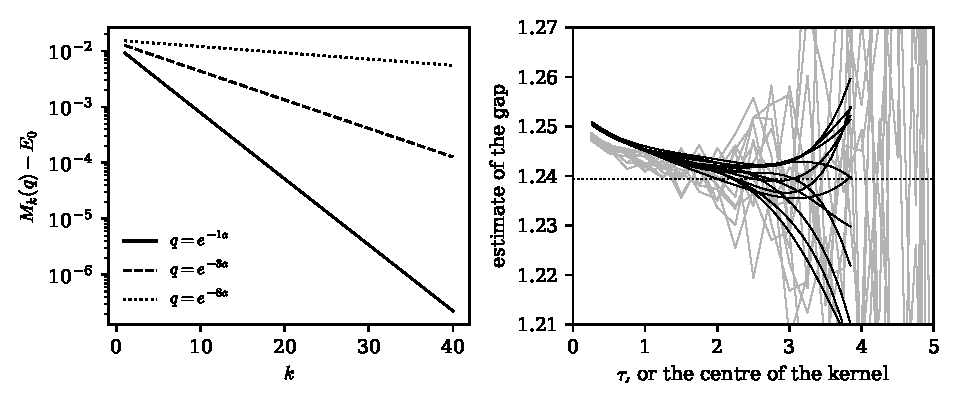
\includegraphics[width=\textwidth]{figures/window_gap.pdf}
\caption[A monotone estimator of the gap]{Left: the excess of $M_k(q)$ over the gap for the exact correlator, for three values of $q$; it is positive and decreasing, as Proposition~\ref{prop:windowgap} says. Right: twelve noisy replicates of the effective mass (grey) and of $M_k$ with $q=e^{-3a}$ (black) against the time at which the kernel is centred; the dotted line is the gap.}
\label{fig:windowgap}
\end{figure}

At matched bias the kernel estimator has about half the noise of the effective mass at short times, a little less at moderate times, and more at long times, where its kernel reaches into the region in which the signal is below the noise. So it is a modest tool with one real merit: every $M_k$ is a rigorous upper bound for the gap, and the sequence is monotone, whatever the spectrum.

\paragraph{\normalfont\scshape Why the kernels are the same.} The localising kernel $u^ke^{-\sigma u}/k!$ of \cite{DLCL} is, after normalisation, the density of a gamma variable of shape $k+1$, the kernel of the inversion formula of Post and Widder~\cite{Pt30,Wi41}, and the negative binomial weight $\binom{j+k}{k}q^j$ is its lattice form: the law of the number of failures before the $(k+1)$st success. Both are convolution powers of one law, exponential or geometric, and both concentrate at relative width $k^{-1/2}$. In the language of this book the first is the simplest generalized gamma convolution and the second its lattice analogue, and the estimator $M_k$ is a ratio of two expectations of the correlator under them. The edge of the support of a positive measure is the limit of ratios of its moments.

\paragraph{\normalfont\scshape A positive selector.} In \cite{DLCL} the functions for different characters are combined with strictly positive coefficients, so that a zero of any one of them is a pole of the sum and cannot cancel. The same device is available here and is equally cheap: a positive combination of reflection positive correlators over channels, for instance $\sum_nc_n\langle\chi_n(U_p)(0)\,\chi_n(U_p)(\tau)\rangle$ with $c_n>0$, has a spectral measure that is the sum of those of its terms, and its gap is the smallest of theirs.

\paragraph{\normalfont\scshape Frames and mean slopes.} The third mechanism is the one the account marks as specific to the construction. There are many maps $J_i$ from small hermitian lattices into one large one, and what is needed is that their images, taken together, fill the target. The step in finite dimensions is the following. It is stated and proved in the exposition \cite{Rub26} of the next section (Part II, section 6.9); we give the proof because it is short and contains no arithmetic. Write $\|A\|_2^2=\operatorname{tr}(A^*A)$.\index{frame lemma}

\begin{lemma}[frame lemma]\label{lem:frame}
Let $J_i:V_i\to H$ be linear maps of complex inner product spaces of finite dimension, with $D=\dim H$ and $W=\sum_i\dim V_i$, and let $c_i>0$. Put $K_i=c_iJ_i^*J_i$ on $V_i$ and $Q=\sum_ic_iJ_iJ_i^*$ on $H$. Then
\[
\operatorname{rank}Q\ \ge\ \frac{(\operatorname{tr}Q)^2}{\operatorname{tr}(Q^2)}.
\]
Suppose further that
\[
\sum_i\|K_i-1\|_2^2\le eW,\qquad e\le\tfrac14,\qquad\operatorname{tr}(Q^2)\le(1+\eta)\,\frac{(\operatorname{tr}Q)^2}{D},
\]
and let $U_i\subset V_i$ be subspaces with $\sum_i(\dim V_i-\dim U_i)\le\alpha W$. Then
\[
\operatorname{codim}\sum_iJ_iU_i\ \le\ \big(\eta+4\alpha+4\sqrt e\,\big)D.
\]
\end{lemma}

\begin{proof}
The first statement is the Cauchy and Schwarz inequality for the nonzero eigenvalues of $Q$. For the second we may take $\alpha\le1$. Let $P$ be the orthogonal projection of $H$ onto the complement of $\sum_iJ_iU_i$, of dimension $zD$. The operator $A_i=c_iJ_i^*PJ_i$ is nonnegative, is at most $K_i$, and vanishes on $U_i$. So with $R_i$ the projection of $V_i$ onto the complement of $U_i$, of rank $r_i$,
\[
\operatorname{tr}A_i=\operatorname{tr}(R_iA_i)\le\operatorname{tr}(R_iK_i)=r_i+\operatorname{tr}\big(R_i(K_i-1)\big)\le r_i+\sqrt{r_i}\,\|K_i-1\|_2.
\]
Summing, and using the Cauchy and Schwarz inequality over $i$,
\[
\operatorname{tr}(PQ)=\sum_i\operatorname{tr}A_i\le\big(\alpha+\sqrt{\alpha e}\,\big)W,
\]
\[
\operatorname{tr}Q=\sum_i\operatorname{tr}K_i\ge\big(1-\sqrt e\,\big)W\ge\tfrac12W.
\]
Let $\bar q=\operatorname{tr}Q/D$. The hypothesis on the second moment says $\|Q-\bar q\|_2^2\le\eta(\operatorname{tr}Q)^2/D$, so
\[
\operatorname{tr}(PQ)=\bar q\,zD+\operatorname{tr}\big(P(Q-\bar q)\big)\ge\big(z-\sqrt{\eta z}\,\big)\operatorname{tr}Q.
\]
Dividing by $\operatorname{tr}Q$ and using $\sqrt{\eta z}\le\frac12(\eta+z)$ gives $z\le2\alpha+2\sqrt e+\frac12(\eta+z)$, which is the claim.
\end{proof}

The two hypotheses say that the maps form an approximate tight frame: each $c_iJ_i^*J_i$ is close to the identity on average, and the frame operator $Q$ is close to a scalar in mean square. The conclusion is a pooled local to global principle. What holds on most of each piece holds on most of the whole. Two maps onto the two axes of $\mathbb C^2$ have $Q=1$ and fill the plane; two maps onto the same axis have the same trace, twice the second moment, and fill a line.

The constants can be improved, and the improved form is sharp.

\begin{proposition}[sharp form]\label{prop:framesharp}
In Lemma~\ref{lem:frame} assume only $e<1$, and put $\rho=(\alpha+\sqrt{\alpha e}\,)/(1-\sqrt e\,)$. Then
\[
\operatorname{codim}\sum_iJ_iU_i\ \le\ \tfrac14\Big(\sqrt\eta+\sqrt{\eta+4\rho}\,\Big)^2D\ \le\ (\eta+2\rho)\,D.
\]
For a tight frame of isometries, $e=\eta=0$, the bound is $\alpha D$, and it is attained.
\end{proposition}

\begin{proof}
The proof of the lemma gives $z-\sqrt{\eta z}\le\operatorname{tr}(PQ)/\operatorname{tr}Q\le\rho$, a quadratic inequality in $\sqrt z$ whose solution is the first bound; the second follows from $\sqrt{\eta^2/4+\eta\rho}\le\eta/2+\rho$. For $e\le\frac14$ and $\alpha\le1$ one has $2\rho\le4\alpha+4\sqrt e$, which recovers the lemma. An orthogonal decomposition $H=\bigoplus_iV_i$ with the inclusions as maps is a tight frame of isometries with $W=D$, and removing a proportion $\alpha$ of the directions of the pieces removes exactly $\alpha D$ directions of $H$.
\end{proof}

In random trials (\texttt{frame\_lemma.py}), $270$ configurations with up to eight maps into spaces of dimension up to forty, neither bound was violated. The lemma as stated says something, a bound below $D$, in $23$ of them, and the sharp form in $58$.

The second step turns a count of directions into a bound for an average.

\begin{corollary}[few low states]\label{cor:lowstates}
Under the hypotheses of Lemma~\ref{lem:frame} on $J_i$, $c_i$, $e$ and $\eta$, let $T$ be a self adjoint operator on $H$ with $T\ge a-L$, where $L\ge0$. Suppose that for each $y\in[0,L]$ there are subspaces $U_i(y)\subset V_i$, of total codimension at most $\alpha(y)W$, with $\langle Tw,w\rangle\ge(a-y)|w|^2$ for every $w$ in $\sum_iJ_iU_i(y)$. Then the number $N(y)$ of eigenvalues of $T$ below $a-y$ is at most $(\eta+4\alpha(y)+4\sqrt e\,)D$, and
\[
\frac{\operatorname{tr}T}{D}\ \ge\ a-\big(\eta+4\sqrt e\,\big)L-4\int_0^L\alpha(y)\,dy.
\]
\end{corollary}

\begin{proof}
If $T\ge\lambda$ on a subspace of codimension $r$ then $T$ has at most $r$ eigenvalues below $\lambda$, since the span of more than $r$ such eigenvectors would meet the subspace. With the lemma this bounds $N(y)$. For the mean, with eigenvalues $\lambda_j$,
\[
\frac{\operatorname{tr}T}{D}\ \ge\ a-\frac1D\sum_j(a-\lambda_j)_+=a-\int_0^L\frac{N(y)}{D}\,dy,
\]
the layer cake formula.
\end{proof}

In \cite{Rub26} the function $\alpha$ comes from Markov's inequality: if numbers with mean at least $s$ are all at most $s+u$, the proportion of them below $s-y$ is at most $u/(u+y)$. Then $4\int_0^L\alpha=4u\log(1+L/u)$, a logarithmic loss in the spread $u$, and the mean slope of the sources is carried to the target. There the operator is a slope and its filtration is that of Harder and Narasimhan~\cite{HN75}; that filtration is what makes a bound on each image a bound on their sum, and the draft says it takes it from the Lean development.

It is fair to say what this would and would not give here. The corollary bounds $\operatorname{tr}T/D$, an average over the spectrum: with $T$ the logarithm of a transfer matrix on a finite block this is a free energy, and for loops a string tension, a rate per unit area. A gap is a statement about the bottom of the spectrum, a set of relative dimension zero, and a bound that allows a small proportion of exceptions cannot see it. So the frame mechanism is a candidate for transferring string tensions under blocking, where the sandwich of Chapter~\ref{ch:sandwich} asks for exactly a comparison of averaged rates, and not for the gap itself. The hypothesis that carries the weight is the form bound on the sum $\sum_iJ_iU_i(y)$, which involves cross terms between the pieces. For blocks of a lattice we do not know what supplies it, and we have not tried.

\paragraph{\normalfont\scshape The budget.} The exponent $\frac12$ comes out in \cite{DLCL} as a balance between a gain repeated along a tower of length $m$ and costs that grow with $m$ in another way. The next section gives its explicit form and the form it takes for the ladder.

We read sections 1, 2 and 5 of \cite{DLCL} in full and part of section 6, and only the headings of the rest; the copy we read names no author. Its arithmetic is taken as stated.

\section{The inequality (M) and the three scales}\label{sec:ineqM}\index{inequality (M)}\index{Chebyshev, P. L.}

The argument for the zeta function alone is set out in a working draft written at the behest of M. O. Rubinstein \cite{Rub26}, which our deck \cite{PS26m} follows. It reduces the Riemann hypothesis to three inputs, and it is explicit about which of them it proves. The statistic is a smoothed Chebyshev sum with its main term removed,
\[
G(x)=\sum_{n\le x}\Lambda_{\mathrm{vM}}(n)\Big(\frac xn-1\Big)-x\log x+(1+\gamma_E)x
=\log2\pi-\sum_{\varrho}\frac{x^{\varrho}}{\varrho(\varrho-1)}+O(x^{-2}),
\]
the sum being over the zeros in the strip, and the criterion is the one sided window of the last section: if $G(x)\le x^{1/2+\varepsilon}$ on intervals $[Y,Y^{3/2}]$ with $Y$ arbitrarily large, there is no zero to the right of the critical line. Two auxiliary primes $q$ and $d$ give the combination $(1+\chi_q)(1-\chi_d)$, whose weight $1-\chi_d$ is nonnegative and selects the primes inert in $\mathbb Q(\sqrt{-d})$. Then:
\begin{itemize}
\item Estimate B, at the scale $x$, far below the conductors: square root bounds for the three twisted sums;
\item Estimate C, at scales far above the conductors: bounds with an exponential saving, from the classical zero free region, for the characters of the table of cells;
\item the inequality (M), an averaged one sided comparison of a prime sum $P$ with nonnegative weights, cut off cell by cell, against its main term $M$, with $B$ the bound of Estimate B,
\[
\frac1n\sum_{u\in H}\sum_{v\in T}\sum_{j\le m}\big(P_{u,v,j}-M_{u,v,j}\big)\le E,
\]
\[
\frac EB\le x^{c_0\varepsilon}\Big(\frac xm+\frac{xm}{k}+m+\frac{k}{n^2}\Big),
\]
with $c_0$ a constant fixed in the draft;
\end{itemize}
B and C are proved in the draft from published theorems on Dirichlet $L$ functions. The inequality (M) is not: the draft proves parts of it, proves others conditionally on named statements, and says it takes the rest from the Lean development. In the table of cells behind (M) a small proportion of distinguished cells tests the primes at the scale $x$ and carries the main term, and every other cell sits at a scale so large that Estimate C makes it negligible.

\paragraph{\normalfont\scshape Divisibility against size.} The source of every upper bound in the argument is Chebyshev's: a nonzero integer divisible by $p^{e_p}$ for each $p$ is at least $\prod p^{e_p}$. For the middle binomial coefficient this bounds the primes between $n$ and $2n$, and it stalls at constants because the exponents of a factorial are floor functions. The draft replaces the integer by a linear map $T:L\to M$ between lattices. If $T$ is injective and $T(L)\subset p^eM$ then
\[
e\log p\ \le\ \log\|T\|+\mu_{\max}(M)-\mu(L),
\]
where the slope $\mu$ of a lattice is minus the logarithm of its covolume divided by its rank, and $\mu_{\max}(M)$ is the largest slope of a nonzero sublattice of $M$; for $L=M=\mathbb Z$ this is Chebyshev's inequality. The maps are theta lifts between definite unitary groups, which are matrices of derivatives of theta functions. At an inert prime a derivative of order $a$ is divisible to the smooth exponent $a(1/p+1/p^3+\cdots)$, with no floor function, and its squared size is that of the Gaussian integral $\|z^a\|^2=a!$. The two sides, summed over the primes, then agree to leading order $a\log a$, and (M) is the statement that they agree in the term linear in $a$ as well, up to $E$.

\paragraph{\normalfont\scshape The budget.} The four terms have different origins (\cite{Rub26}, section I.8). The term $x/m$ collects errors made once, in the sizes of the lattices at the two ends of a chain of $m$ lifts: the gain from divisibility is collected $m$ times, so they are divided by $m$. The term $m$ collects errors made at every step. The terms $xm/k$ and $k/n^2$ are the costs of a rank $k$ and of the size $n$ of the table. With $m=x^{1/2}$, $k=x^{9/2}$ and $n=x^2$, up to powers of $x^\varepsilon$, the terms are $x^{1/2}$, $x^{-3}$, $x^{1/2}$ and $x^{1/2}$. That is why the exponent is one half. Had the errors of the steps cost $m^2$ after normalisation, the balance of $x/m$ against $m^2$ at $m=x^{1/3}$ would give only the half plane to the right of $\frac23$; the precision of the comparison of lattices decides the exponent.

We have read Part I of the draft, the sections of Part II on slopes and ranks, and the table of what Part III proves; we have not read the proofs of Part III. With that said, the architecture resembles what one would expect of a proof of the mass gap, and the correspondence is close enough to set out.

\begin{center}
\small
\begin{tabular}{p{0.46\textwidth}p{0.46\textwidth}}
\toprule
the argument through (M) & the mass gap \\ \midrule
Estimate B: below the conductor the characters behave like random signs, square root cancellation & weak coupling at short scales: asymptotic freedom, the renormalisation group of Ba\l aban \cite{Ba87}, the first rungs of the ladder \\
Estimate C: far above the conductor a classical zero free region gives an exponential saving & strong coupling at long scales: the convergent expansion of Osterwalder and Seiler \cite{OSe} gives an area law and a gap \\
(M): the bridge between the two scales, one sided and averaged & the comparison at intermediate coupling, Chapter~\ref{ch:sandwich} \\
the one danger in C is an exceptional real zero, avoided by the choice of $q$ and $d$ & the one danger is a phase transition at intermediate coupling; on the projected ladder Corollary~\ref{cor:contracts} excludes it \\
nonnegative weights $1-\chi_d$ & the nonnegative action $1-\frac12\operatorname{tr}U=2\sin^2(\theta/2)$ and reflection positivity \\
distinguished cells carry the main term, the rest are killed by C & blocks at the scale of the correlation length carry the gap, coarser ones are in the strong coupling phase \\
budget $x/m+xm/k+m+k/n^2$, balanced at $x^{1/2}$ & a drift per rung against an error per rung (below, and Open problem~\ref{op:slopes}) \\
(M) is, by the draft, taken in part from the Lean development & existence is quoted from an announced proof, not checked by us (Section~\ref{sec:existence2026}) \\
\bottomrule
\end{tabular}
\end{center}

Two things in this are more than analogy. The first is the logic. Both ends of the scale are classical in both problems, and in both the whole difficulty is a one sided inequality across the middle. Proposition~\ref{prop:windowgap} says that for the gap one sidedness and sparseness are free, so the statement to prove has the following form.

\begin{problem}[an inequality of type (M) for the ladder]\label{op:MYM}
For SU(2) lattice gauge theory in four dimensions at coupling $\beta$, let $c_n$ be the count $E[1/(1-\frac12\operatorname{tr}U)]-2$ of the plaquette of the lattice blocked $n$ times with scale factor $2$, and $\ell_n$ the count after $n$ exact rungs of the ladder from the law of the fine plaquette. Prove $c_n\le\ell_n+E_n$ with an error $E_n$ small enough that $\ell_n+E_n$ still falls below the threshold of the strong coupling expansion after a number of blockings proportional to $\beta$. Only an upper bound is asked, and only along the sequence of scales $2^n$.
\end{problem}

\paragraph{\normalfont\scshape The budget of the ladder.} The ladder has the same two kinds of error and a different arithmetic. Suppose that $c_n\le\ell_n+e_0+e_1n$, with an error $e_0$ made once and an error $e_1$ made at every rung, and that the count on the ladder falls by $\delta$ per rung, $\ell_n\le\ell_0-\delta n$. Then
\[
c_n\le c_*\qquad\text{as soon as}\qquad n\ \ge\ \frac{\ell_0-c_*+e_0}{\delta-e_1}.
\]
In (M) the gain grows with the length of the chain and is set against costs that grow too, and the optimum is interior. Here the gain is a fixed drift, so there is no optimum and one condition: $e_1<\delta$, the error per rung must be smaller than the drift. An error made once costs $e_0/(\delta-e_1)$ further rungs, a fixed factor in the scale, and is harmless.

The numbers at weak coupling are these. The plaquette of the four dimensional lattice has $1-\langle\frac12\operatorname{tr}U_p\rangle=3/(4\beta)$ to leading order, and its field strength is Gaussian in three components, for which $E[1/(1-x)]=3/E[1-x]$. So $\ell_0=c_0=4\beta$ to leading order, twice the count $2\beta-\frac32$ of a Wilson law at the bare coupling: the plaquette in four dimensions is stiffer than its action alone would make it. The drift is $\delta=\frac12$, a numerical observation for heat kernels (Theorem~\ref{thm:firstrung} proves the first rung only for point masses and Wilson laws, and the limit $r\to\frac13$ that gives $\frac12$ is unproved). With no error the ladder from the fine plaquette therefore needs about $8\beta$ rungs, a scale $2^{8\beta}=e^{5.55\beta}$, while asymptotic freedom puts the correlation length at $e^{3\pi^2\beta/11}=e^{2.69\beta}$ up to a power of $\beta$, about $3.9\beta$ blockings. So $c_n\le\ell_n$ has room at weak coupling: the true count must fall about twice as fast as the ladder's, and $e_1$ may be taken negative. The ladder from the bare Wilson law, by contrast, needs $4\beta$ rungs against $3.9\beta$, the agreement of the decrement $\frac14$ with $0.26$ noted in Chapter~\ref{ch:sandwich}; but its count starts below $c_0$, and the inequality fails for it at $n=0$.

Two cautions belong with these numbers. The leading order is not yet accurate at the couplings we can simulate: at $\beta=2.3$, $2.5$ and $2.7$ the measured $E[1/(1-x)]$ is $7.2$, $8.3$ and $9.2$ against $4\beta=9.2$, $10.0$ and $10.8$, a ratio that rises from $0.78$ to $0.85$. And the comparison of $8\beta$ with $3.9\beta$ is a comparison of exponents only. It says that the ladder from the fine plaquette reaches strong coupling at a scale near the square of the true one, which is the direction an upper bound must err in, and it says nothing about any finite $n$.

\begin{center}
\small
\begin{tabular}{lccc}
\toprule
 & start & blockings & scale \\ \midrule
ladder from fine plaquette & $4\beta$ & $8\beta$ & $e^{5.55\beta}$ \\
ladder from bare Wilson law & $2\beta$ & $4\beta$ & $e^{2.77\beta}$ \\
asymptotic freedom & & $3.9\beta$ & $e^{2.69\beta}$ \\
\bottomrule
\end{tabular}
\end{center}

The evidence is in Tables~\ref{tab:countblocked} and~\ref{tab:countblocked2}, where the ladder starts from the Wilson law matched to the fine plaquette rather than from the law of the fine plaquette itself. On $16^4$ with two blockings $c_n\le\ell_n$ holds at both levels for $\beta=2.3$ and $2.5$, with a margin that grows with the level, $1.27$ against $4.87$ and $4.00$ against $6.04$ at the second. At $\beta=2.7$ it fails at the first level, $8.14$ against $7.48$, and holds at the second, $6.75$ against $7.01$: a smeared blocking at weak coupling first raises the count. In the terms above that is an error $e_0$ of about $0.7$ made once, and between the first and second levels the lattice count falls by $2.5$, $2.1$ and $1.4$ at the three couplings against $0.47$ on the ladder, so $e_1$ is negative there. This is two rungs on small lattices; it is not an estimate of either error.

The second is the device of averaging. In (M) the average over the translates $u\in H$ is what turns the selection of cells into characters, by orthogonality on a cyclic group. The lattice has the same device with the gauge group in place of $H$: averaging over gauge transformations is what turns products of link variables into characters of plaquettes, and it is how the matching expansion of Theorem~\ref{thm:matching} was obtained. A proof of Open problem~\ref{op:MYM} would presumably use it in the same way, to replace the blocked measure by an average of measures each of which is a product over cells.

\section{What theta lifts do not give}

The engine of the chain is arithmetic: divisibility of theta values at inert primes, a slope inequality that trades it against archimedean size, and the balance of the two that fixes the length of the chain. Yang Mills has none of this. The step that turns a one sided bound into a zero free region needs a Dirichlet series with positive coefficients; the mass gap needs a spectral bound for an operator in infinitely many variables. Induced gauge theories built from flavours change the action, and whether they lie in the universality class of Yang Mills is open by their authors' own account. And everything in this chapter concerns one plaquette or one decimation: the lattice $\mathbb Z^4$ is untouched.

It helps to be exact about where the proof of (M) lives. By the account of \cite{Rub26}, three things have to be established about the lifts: divisibility at inert primes, which rests on the integrality of the theta kernels in the coordinates of a formal group of height two; size to the precision of the linear term, which rests on the inner product formula, the formula of Chowla and Selberg and the mass formula; and control of denominators and of rank, which rests on a bound for Galois cohomology and on a relative trace formula. All of that is arithmetic, none of it has a counterpart for a lattice gauge theory, and the draft says it takes the parts it does not prove from the Lean development. What transfers is what surrounds it: the one sided window, the frame lemma, the passage from a count to a mean, and the shape of the budget. Those are the four things this chapter has taken.

\section{Open problems}

\begin{problem}\label{op:matching}
Prove that the matching expansion of Theorem~\ref{thm:matching} has only real zeros in $x$, all at most $-1$, for hopping parameters in $(0,1]$: a theorem of Heilmann and Lieb type for the variable that marks only the pairs between two blocks of a complete graph. This is Conjecture~\ref{conj:Lclosed}.
\end{problem}

\begin{problem}\label{op:symplectic}
Write the colour flavour transformation for SU(2) as a symplectic group, with the inner pairs, and identify the law of the masses $\lambda_i(Z)$ of the mixture. For all hopping parameters equal to $1$ the answer is the hypergeometric law of the count.
\end{problem}

\begin{problem}\label{op:slopes}
Bound the error per rung $e_1$ of Section~\ref{sec:ineqM} below the drift $\frac12$ of the count, for some blocking of the four dimensional lattice and all $\beta$ large. By the budget of the ladder this, with any bound on the error $e_0$ made once and the drift $\frac12$ at every rung (a numerical observation, with the first rung theorem covering only point masses and Wilson laws), would give Open problem~\ref{op:MYM}. At weak coupling the true count falls about twice as fast as the ladder's, so the bound is expected with room to spare; nothing is proved.
\end{problem}

\section{Assessment}

Useful, as a language and for one open problem. The determinant form explains why the class $\mathcal L$ is natural, why the count is a sum of Bernoulli variables and why the heat kernel belongs to it. The matching expansion is a new exact formula for decimation and brings the closure conjecture within sight of a classical theorem, separated from it by the pairs inside each law. The window criterion of the expanded account becomes, for a positive spectral measure, an elementary proposition and a monotone estimator of the gap. The frame lemma is portable as it stands and bounds averages, not gaps. The budget of (M) becomes one condition for the ladder, an error per rung below the drift. Nothing here is a step toward the gap on $\mathbb Z^4$. We read \cite{PS26t} in full; its account of the arithmetic of the chain is taken from the sources it cites, and so is ours. The colour flavour formula above is quoted from memory of \cite{Zi96} and checked in one case only.

\section*{Exercises}
\begin{enumerate}
\item (Section~\ref{sec:t11det}) Verify $\det(1+\alpha U)=(1-\alpha)^2+\alpha\det(1+U)$ and deduce the Bernoulli parameter $1/\gamma$ of the count from the normalisations $Z_0=1$ and $Z_1=1$.
\item (Section~\ref{sec:t11howe}) From Proposition~\ref{prop:howe} show that $a_1=\sum_qe_q^2-\sum_qe_qe_{q+2}$ and compute it for $\alpha=(1,1)$.
\item (Section~\ref{sec:t11match}) List the matchings of four flavours, two in each law, and recover $f_2*f_2$ from Theorem~\ref{thm:matching}.
\item (Section~\ref{sec:windows}) Prove Proposition~\ref{prop:windowgap}(ii) for a spectral measure with two atoms, and find the rate at which $M_k(q)$ approaches $E_0$ in terms of $q$ and the two energies. Which $q$ makes the approach fastest, and why is that choice useless with noisy data?
\item (Section~\ref{sec:windows}) Prove that $\operatorname{rank}Q\ge(\operatorname{tr}Q)^2/\operatorname{tr}(Q^2)$ for a nonnegative matrix $Q$, and find $\eta$ in Lemma~\ref{lem:frame} for $p$ isometries of $\mathbb C^r$ into $\mathbb C^D$ with orthogonal images and $c_i=1$. When does the lemma say the images fill the target?
\item (Section~\ref{sec:windows}) For numbers with mean at least $s$ and maximum at most $s+u$, show that the proportion below $s-y$ is at most $u/(u+y)$, and that this cannot be improved.
\item (Section~\ref{sec:ineqM}) In the budget of the ladder take $\ell_0=4\beta$, $c_*=1$ and $\delta=\frac12$. For which $e_1$ does the number of rungs equal the $3.9\beta$ blockings of asymptotic freedom at large $\beta$? What does the sign of the answer say about the ladder?
\item (Section~\ref{sec:t11match}) Show that for U(2) the average of $\det(1+\alpha UV^{-1})\det(1+\kappa V)$ over $V$ is $1+\alpha\kappa x+\alpha^2\kappa^2$ for $U$ in SU(2), and compare with the SU(2) convolution. Which terms are the inner pairs?
\end{enumerate}
